\documentclass[12pt,reqno]{amsart}
\usepackage{/Users/johnmyers/GoogleDrive/tex/handout,/Users/johnmyers/GoogleDrive/tex/customcommands,polynom}
\usepackage{caption}

\hdr{MAT 240}{\S16.1 Integrals of functions of two variables}

\begin{document}

\textbf{Suggested problems:} 1-5 odd, 13, 15

\bigskip
\hrule

\bigskip

\prob The contour diagram of a function $f$ is shown below. Estimate $\int_R f \ dA$ if $R$ is the rectangular region with $0 \leq x \leq 30$ and $0 \leq y \leq 15$.


\includegraphics[scale=1.25]{pic1.pdf}

\bigskip
\textcolor{red}{Take $\Delta A =50$, and sample points in the upper left-hand corners of the subrectangles. Then
	\[\int_R f \ dA \approx 50( 4 + 5 + 7 + 6.6+ 7 + 8 + 8.5+ 9 + 10) = 3255.
	\]}
\bigskip


\prob The table below gives the values of $f(x,y)$, the number of milligrams of mosquito larvae per square meter in a swamp. If $x$ and $y$ are in meters and $R$ is the rectangle with $0 \leq x \leq 8$ and $0 \leq y \leq 6$, estimate $\int_R f \ dA$. Give units and interpret your answer.

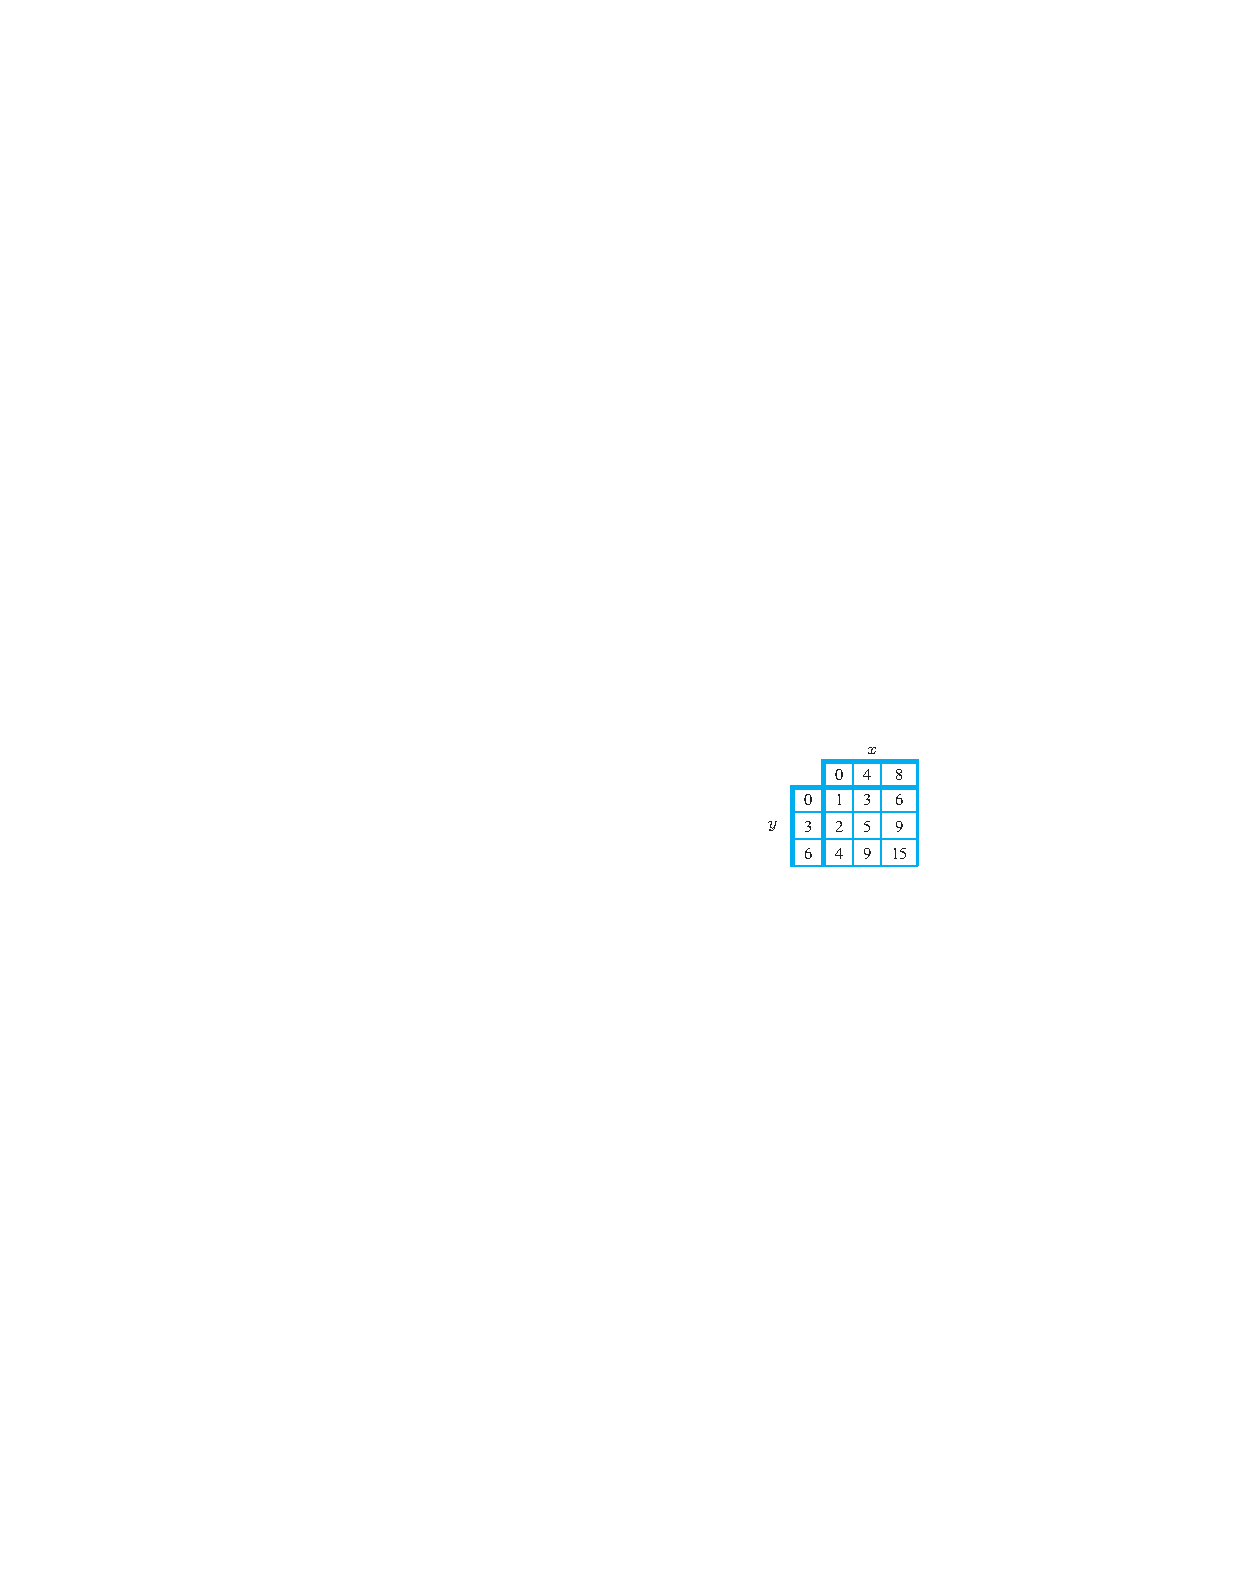
\includegraphics[scale=1.25]{pic2.pdf}

\bigskip
\textcolor{red}{We take $\Delta A = 12$. Then with sample points in the upper right-hand corner, we get
	\[\int_R f \ dA \approx 12 ( 5+9+9+15) = 456 \tn{ mg mosquito larvae.}
	\]}

\bigskip
\textcolor{red}{}
\bigskip

\prob The figure below shows a contour plot of population density, people per square kilometer, in a rectangle of land 3 km by 2 km. Estimate the population in this region.

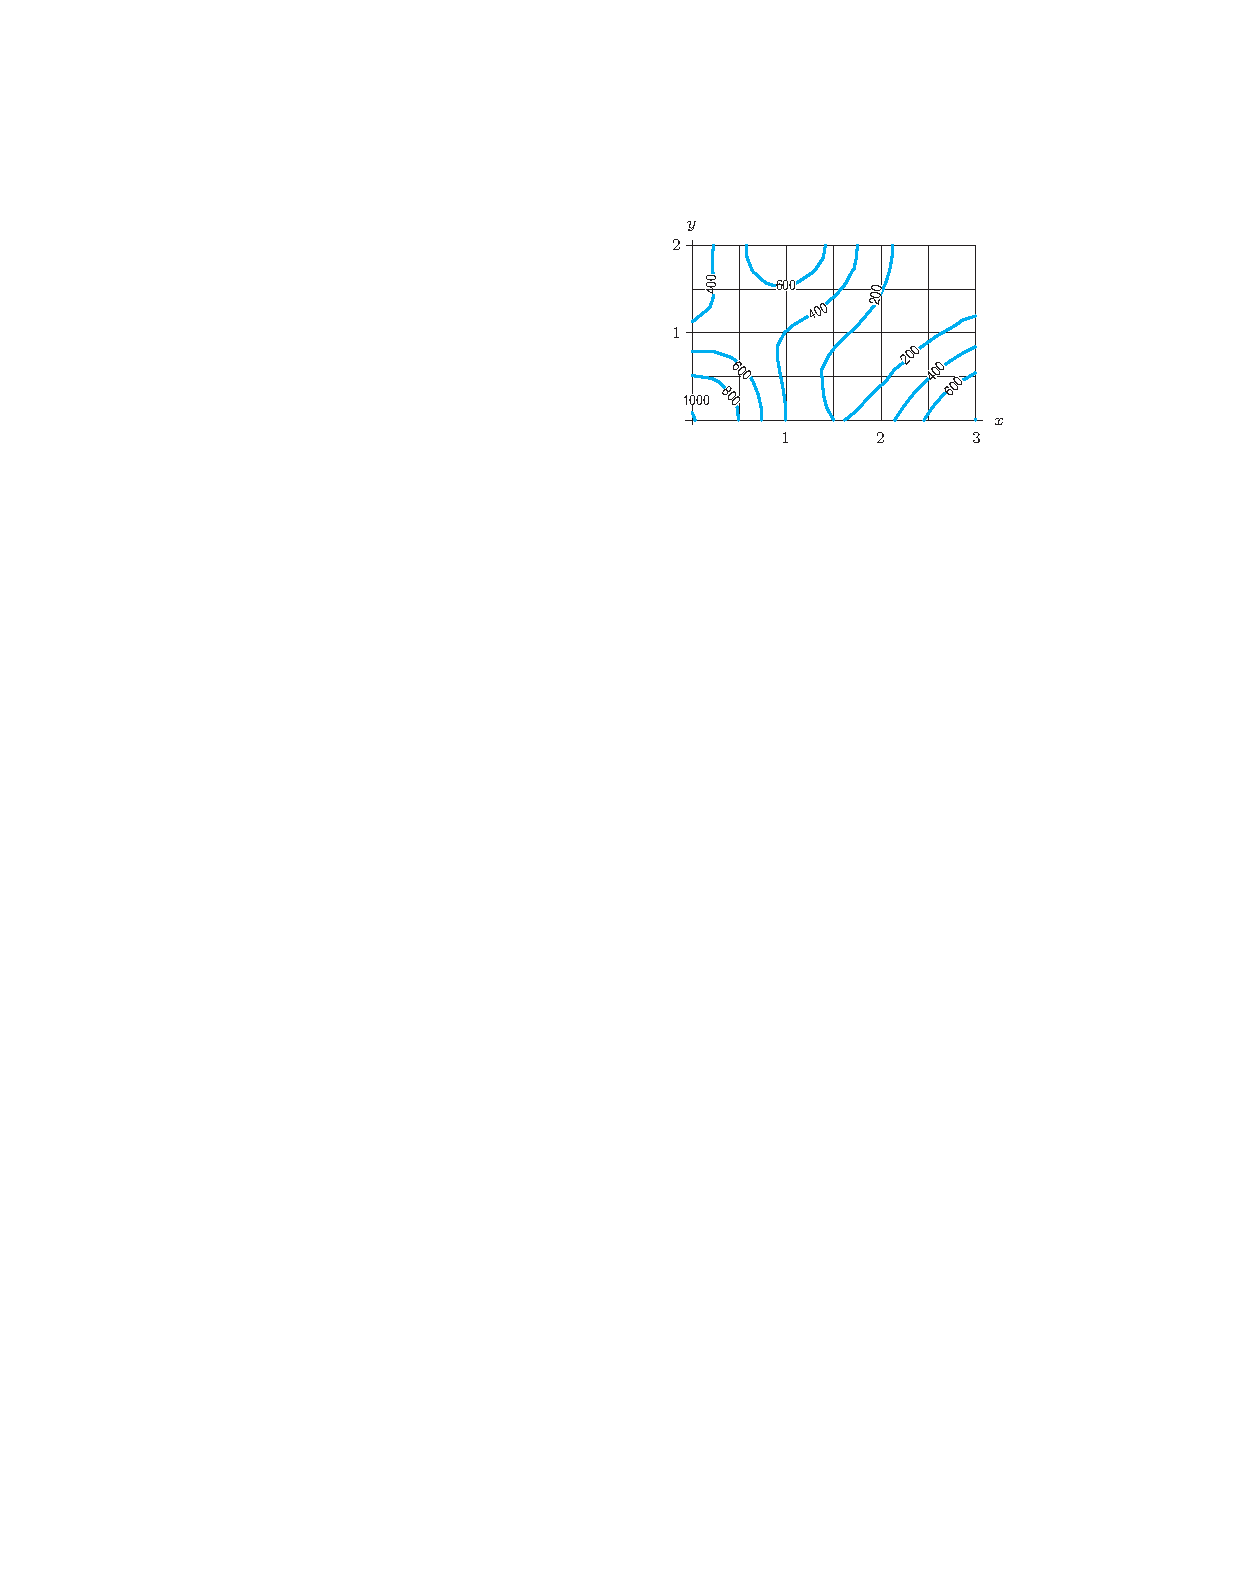
\includegraphics[scale=1]{3.pdf}

\bigskip
\textcolor{red}{We take $\Delta A =1$. If $p(x,y)$ denotes the population density function and $R$ denotes the rectangle of land, then with sample points in the upper right-hand corner, we get
	\[\int_R p  \ dA \approx 1 ( 400 + 100 + 300 + 700 + 250 + 100) = 1850.
	\]
Hence there are approximately 1,850 people in the rectangle of land.}


\bigskip
\prob If $R$ is the rectangle $[0,2] \times [0,4]$, then evaluate
	\[\int_R 2x \ dA.
	\]

\bigskip
\textcolor{red}{From the graph of $z=2x$, we get
	\[\int_R 2x \ dA = 16.
	\]}


\end{document}